\documentclass[tikz]{standalone}

\usepackage{tikz}
\usetikzlibrary{trees}
\usetikzlibrary{shapes}
\usetikzlibrary{positioning}
\usetikzlibrary{arrows.meta}

\tikzset{
    pointer/.style = {thick,draw=black,triangle 45-*,shorten >=-3pt},
    cell/.style = {rectangle, thick, draw=black,minimum width = 1cm, minimum height =1.0cm,fill=yellow!20},
    mynode/.style = {circle, thick, draw=black, align=center,fill=yellow!40,font=\ttfamily\bfseries\Large},
    mynoder/.style = {circle, thick, draw=black, align=center,fill=red!30,font=\ttfamily\bfseries\Large},
    mynodeb/.style = {circle, thick, draw=black, align=center,fill=blue!30,font=\ttfamily\bfseries\Large},
    edgen/.style = {-latex,ultra thick},
    edger/.style = {-latex,ultra thick,red},
    edgeb/.style = {-latex,ultra thick,blue},
    edgeg/.style = {-latex,ultra thick,gray},
    edgegd/.style = {-latex,ultra thick,brown,dashed}, % back
    edgevd/.style = {-latex,ultra thick,violet,dotted}, % forward
    edgexd/.style = {-latex,ultra thick,blue,densely dotted}, % traversal
    every picture/.style={/utils/exec={\ttfamily\bfseries}},
    every picture/.style={font issue=\ttfamily\bfseries},
    font issue/.style={execute at begin picture={#1\selectfont}
  }
}

\begin{document}



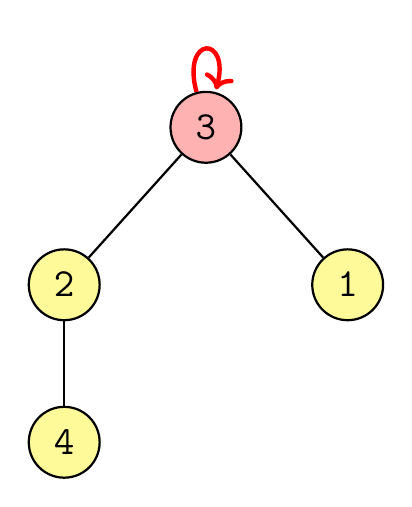
\begin{tikzpicture}[
  thick,
  level distance=2cm,
  level 1/.style={sibling distance=3.6cm},
  level 2/.style={sibling distance=2.4cm},
  level 3/.style={sibling distance=1.2cm},
	font=\ttfamily\bfseries]
  \node[mynoder, minimum size=0.9cm] at (0,0) (a) {3}
    child {node[mynode, minimum size=0.9cm]  {2}
      child {node[mynode, minimum size=0.9cm]  {4}}
    }
    child {node[mynode, minimum size=0.9cm] {1}
    };
  \draw[edger,->] (a) edge[loop above] node {} (a);
 \end{tikzpicture}


\end{document}
